\section{Data Selection}
Collision events were accepted using a hardware trigger which required at least two PMTs fired on each side of the \mbd. In the offline analysis, a set of MB selection criteria has been applied using signals from both the \mbd and \zdc to remove events consistent with beam-related backgrounds and non-hadronic interactions. Figure~\ref{fig:mbdzdc} shows the correlation of energy in the ZDCs to the \mbd charge sum for events passing the MB selection criteria. The \mbd charge sum is the sum of calibrated charge from all PMTs on both sides of the \mbd, and is calibrated such that one MIP is set at unity. A characteristic decrease in the total \zdc energy is observed at both high and low \mbd charge, corresponding to very central collisions (where only a small number of spectator neutrons deposit energy in the \zdc) and to peripheral collisions (where most spectator neutrons are bound in larger nuclear fragments and are thus deflected away from the \zdc by the RHIC magnets), respectively. This analysis utilizes 4.38\ten{6} MB events.

\begin{figure}[t!]
  \centering
  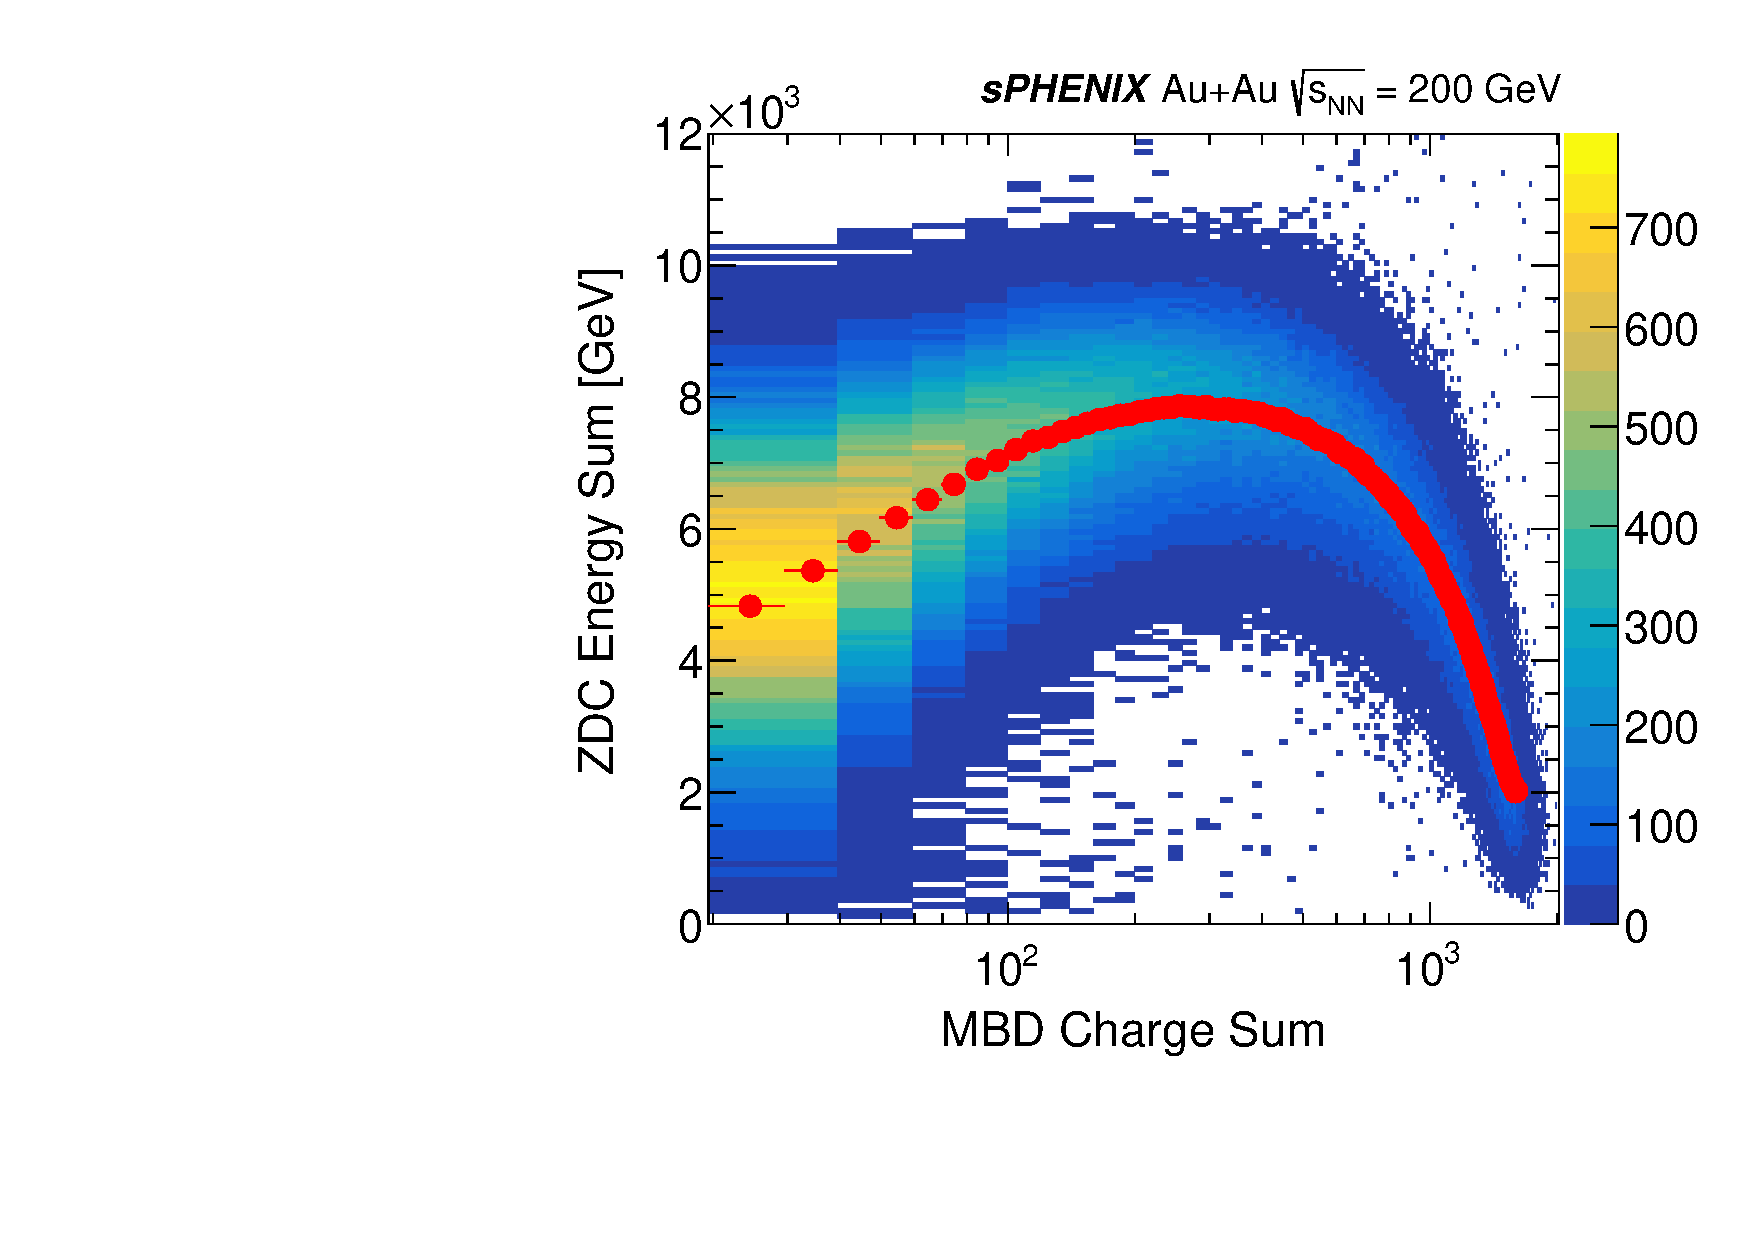
\includegraphics[width=0.5\textwidth]{fig/run54280_charge_sum_zdc.pdf}
  \caption{The correlation between the total energy in ZDCs and the \mbd charge sum is shown. The \mbd charge sum is in units of calibrated MIPs. The red points indicate the average \zdc energy as a function of \mbd charge sum.} 
  \label{fig:mbdzdc}
\end{figure}

The \mbd charge sum is used in each event to assign a centrality value that characterizes the level of geometric overlap between the two colliding nuclei. Centrality percentiles are derived by fitting the \mbd charge sum distribution for all MB events to a model of the particle production and event sampling based on the convolution of a Monte Carlo (MC) Glauber simulation~\cite{Loizides:2014vua} with a negative binomial distribution (MC Glauber $\oplus$ NBD)~\cite{PHENIX:2004vdg,PHENIX:2013jxf}. Figure~\ref{fig:centralityfiv} shows the \mbd charge sum distribution, along with the best fit of the MC Glauber $\oplus$ NBD model and resulting centrality intervals. The bottom panel of Figure~\ref{fig:centralityfiv} shows the peripheral event region to highlight the MB trigger efficiency turn-on region. The total MB selection efficiency for inelastic Au+Au events is then determined by comparing the integral of the data distribution to the integral of the MC Glauber $\oplus$ NBD, normalized for \mbd charge sum $>150$. The resulting efficiency is $92.0\%^{+3.4\%}_{-3.1\%} (\text{syst.)}$, similar to previous \auau data-taking in \phenix where the \mbd was in a different location~\cite{PHENIX:2004vdg}. Glauber model parameters for \auau collisions at $\sqrtsnn=200\gev$ are shown in Table~\ref{tab:glauber}. 

\begin{figure}[t!]
  \centering
  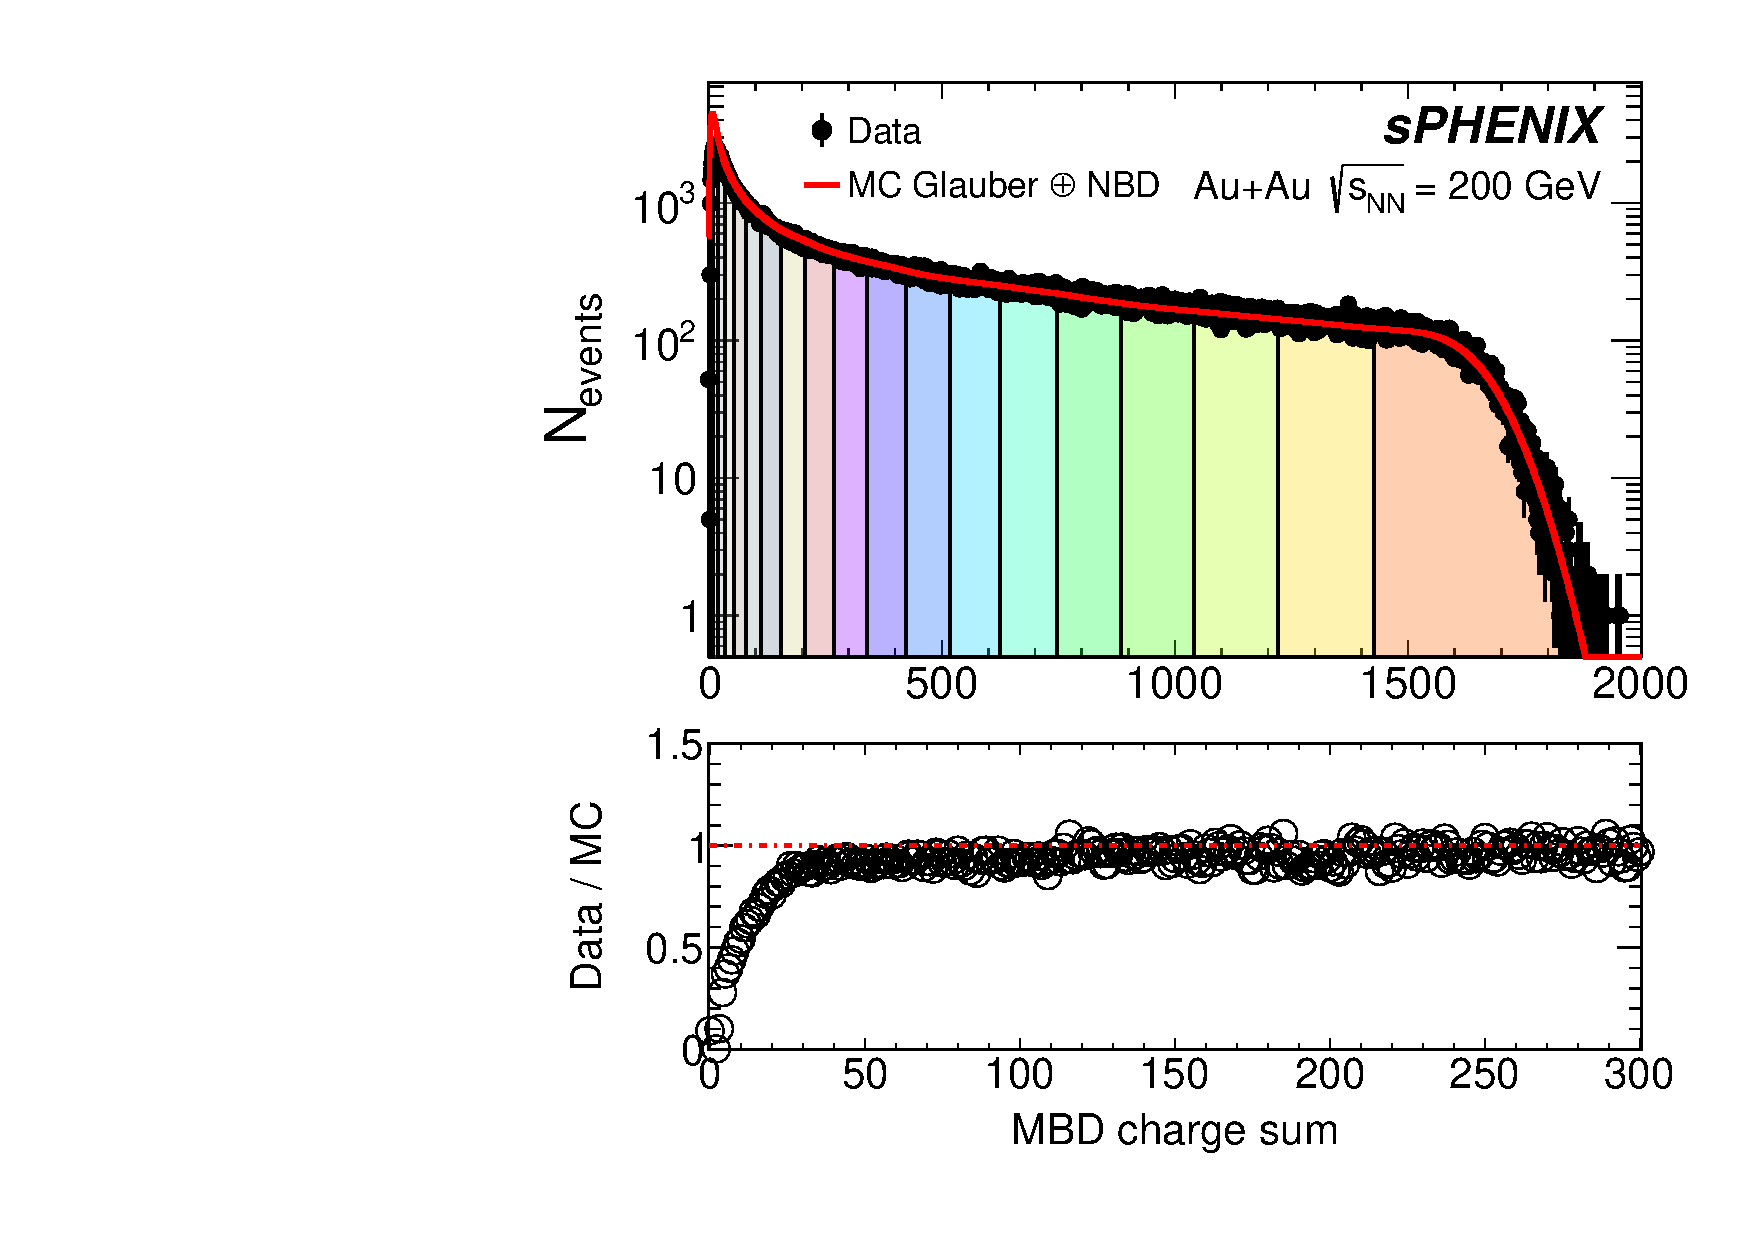
\includegraphics[width=0.5\textwidth]{fig/run54280_glauber_bal.pdf}
  \caption{Top panel: the distribution of total charge deposited in the \mbd (solid black circles), the best fit of an MC Glauber model convolved with an NBD (red line), and centrality intervals for the MB events of \auau collisions at \sqrtsnn=200\gev collected with zero magnetic field (shaded regions). Bottom panel: the trigger efficiency as a function of the \mbd charge deposit in the peripheral collision region.} 
  \label{fig:centralityfiv}
\end{figure}

\begin{table}[H]
    \centering
    \caption{Glauber model parameters for \auau collisions at $\sqrtsnn=200\gev$.}
    \begin{tabular}{l c}
        \toprule[1pt]
        \textbf{Glauber model parameter} & \textbf{Value} \\
        \midrule[1pt]
         $\sigma_{NN}$ [mb] & $42\pm3$ \\[2mm]
         Nuclear radius [fm] & $6.38^{+0.27}_{-0.13}$ \\[2mm]
         Skin depth [fm] & $0.535^{+0.020}_{-0.010}$ \\
         \bottomrule[1pt]
    \end{tabular}
    \label{tab:glauber}
\end{table}

% The hardware MB trigger requires that at least two PMTs fired on each side of the \mbd. 
% In the offline analysis, an additional set of MB selection criteria is applied based on correlations between signals in the \mbd and \zdc to remove non-collision backgrounds and non-hadronic interactions.
% The selection efficiency is determined to be $92.0\%^{+3.4\%}_{-3.1\%} (\text{syst.)}$, obtained by the ratio of the integral of the \mbd charge sum distribution and the simulated multiplicity distribution assuming inelastic collisions.

% Centrality determination
% The event centrality, characterizing the overlap of the two nuclei at the moment when they interact, is determined from the total charge deposit measured in the \mbd. Assuming a monotonic relationship between detector response and event activity, the charge distribution is fitted to a model of particle production and event sampling. This model is based on the convolution of a Monte Carlo (MC) Glauber simulation~\cite{Loizides:2014vua} with a negative binomial distribution (NBD), establishing a correlation with \npart. The charge distribution is then divided into equal intervals, with each bin representing a percentile of the total nuclear interaction cross-section. Events in the highest-multiplicity bin correspond to the most central collisions, which have the smallest impact parameters. The inelastic nucleon-nucleon cross-section is assumed to be $42.0\pm3.0$\mbarn, with a nuclear radius $6.4^{+0.3}_{-0.1}\fm$ and the Woods-Saxon skin depth of $0.535^{+0.020}_{-0.010}\fm$. Figure~\ref{fig:centralityfiv} shows the total charge distribution in the \mbd, the best-fit MC Glauber model convolved with an NBD, and the corresponding centrality intervals. The bottom panel presents the trigger efficiency in the peripheral collision region, emphasizing the transition to full efficiency.

A z-vertex cut, $|z_\mathrm{vtx}|\leqslant10\cm$ determined by the \intt, is imposed, ensuring the collisions take place in the position where the designed acceptance of the \intt can be maintained.
The \intt z-vertex is determined using tracklets, as described in Section~\ref{sec:analysis}. %The resolution of the \intt z-vertex is measured to be 1.7\mm within the selected centrality interval. 

Three different MC event generators, \hijing, \ampt, and \epos, are used in this analysis to determine correction factors for extracting \dndeta from the \sphenix \intt measurement. \hijing, a Heavy Ion Jet Interaction Generator, is used to obtain the nominal results, while \ampt and \epos serve as alternative models to assess the uncertainty in the corrections due to differences in physics modeling.
\hijing models initial parton scatterings using perturbative QCD, describes jet fragmentation and hadronization with the Lund string model~\cite{ANDERSSON1987289}, and applies the Dual Parton Model~\cite{Capella:1992yb} to simulate soft interactions. It also incorporates effects such as jet quenching and nuclear shadowing in parton distribution functions. A Multi-Phase Transport model (\ampt) includes explicit interactions between initial minijet partons and final-state hadronic interactions. It extends \hijing by evolving initial partons with Zhang's parton cascade (ZPC) procedure~\cite{Zhang:1997ej} and the ART model~\cite{Li:1995pra} for the last stage of parton hadronization. \epos, based on Gribov-Regge theory~\cite{gribov1968reggeon, Drescher:2000ha}, includes nuclear effects such as Cronin transverse momentum broadening, parton saturation, screening, as well as high-density effects that lead to collective hadronization in hadron-hadron scattering.

The detector response is simulated using \geant~\cite{Geant4_cite} and processed through the same event reconstruction chain as the data. The \intt geometry in the detector simulation is adjusted based on survey measurements conducted after the \intt was installed in its current position within \sphenix. Simulations are generated using a vertex distribution with the mean and width set to match those observed in the collision data.

In line with previous measurements at RHIC and LHC~\cite{ALICE-PUBLIC-2017-005}, the primary charged hadrons are defined as prompt charged hadrons produced directly in the strong interaction and decay products of particles with proper decay length $c\tau < 1 \cm$, where $c$ is the speed of light in vacuum and $\tau$ is the proper lifetime of the particle. This definition excludes contributions from leptons, decay products of particles with longer lifetimes (such as $K_{S}^{0}$, $\Lambda$), and secondary interactions.